
\section{Features}
In this section, we propose some features which are useful to develop two predictors of how much funding and the number of backers. We groups all our proposed features in different traits:
\subsection{Project-based features}
Given a Kickstarter project's page, we extracted all following features:
\begin{itemize}
	\item number of project's comments,
	\item number of updates
	\item number of rewards,
	\item number of images,
	\item number of videos,
	\item number of faqs,
	\item the goal of the project
	\item category of the project
	\item duration of fund raising of the project
	\item smog score of all rewards: we extracted all rewards' description of the Kickstarter project then grouped them into one document. Next, we computed the smog score of the document and considered it as smog score of all rewards' description.
	\item number of reward sentences,
	\item number of main sentences,
	\item smog score of project's description: we extracted the project's description and computed its smog score.
	\item smog score of biography description
\end{itemize}
SMOG score of a document show how well the document is written. The higher the SMOG score, the better the document was written. The formula to compute SMOG score is as following:
\[
	grade = 1.0430\sqrt{\#polysyllables * \frac{30}{\#sentences}} + 3.1291	
\]
\subsection{Creator-based features}
We proposed some features related to Kickstarter creators as following:
\begin{itemize}
	\item successful rate of all previous backed projects: given a Kickstarter project, we collected all projects that the creator backed and calculate the average successful rates of these backed projects. Our intuition behind it is that if the creator backed many successful projects, he may have an idea of how to get more fund and attract more backers.
	\item previous successful rate of creator's project: we first collected all projects that the creator launched. Then we calculate average successful rate of such projects. The intuition is that if the creator successfully raised fund in many projects, he may have many experience in raising more fund or getting interest from backers.
	\item number of created projects: as mentioned in \cite{chung2015long}, the more projects that creator launched, the more successful he is in raising fund.
\end{itemize}
\subsection{Social network - based features}
Social promotion is an effective way to promote Kickstarter project and attract more funding. Hence, we use some features related to social communication of the creator as following:
\begin{itemize}
	\item number of Facebook friends
	\item connected to Twitter? (binary feature)
	\item connected to Facebook? (binary feature)
	\item connected to Youtube? (binary feature)
	\item how many websites that the creator has?
\end{itemize}
\subsection{Feature Selection}
In this section, we present our approach to remove non-significant features. We first remove all highly correlated features by setting cutoff value of 0.7. That is, if a feature has correlation score of greater than or equal to 0.7 with another one, we remove such feature. After removing all the highly correlated features, we obtained the correlation matrix as shown in Figure \ref{fig:CorrelationMatrix}. 

Among all the rest of uncorrelated features, we would like to keep only significant features. In order to do so, we sequentially choose p features (p = 1,..,n) and calculate the stepAIC value as following:
\[
	stepAIC = nln(SSE_p) - nln(n) + 2p
\]
where \emph{n} is the total number of features, $SSE_p$ is the sum of square error (SSE) that we got by building the model with \emph{p} features. We will choose the subset of all n features which minimize stepAIC score.

\begin{figure}%[!ht]
	\centering
	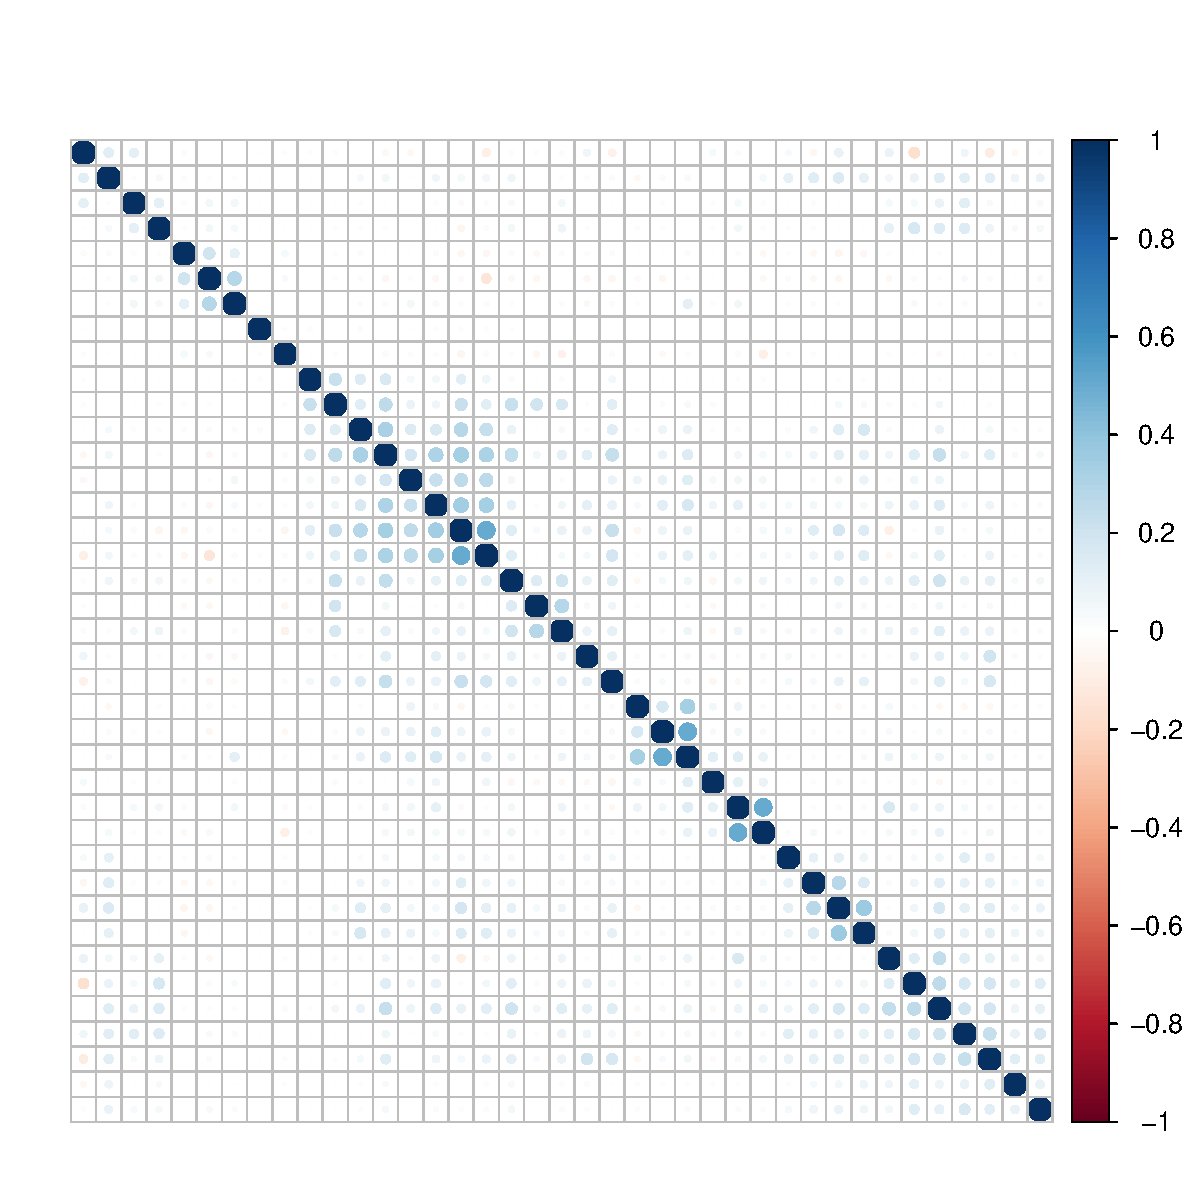
\includegraphics[width=\linewidth]{figs/CorrelationMatrix.pdf}
	\caption{Correlation matrix of all features after removing highly correlated features}
	\label{fig:CorrelationMatrix}
	\vspace{-10pt}
\end{figure}

\section{Our proposed non-linear Regression model}
Fitting a linear model for our problems of predicting the number of backers and the amount of funding for a given Kickstarter project may not be always helpful since the correlation between all features and response could not be linearity.  Hence, we proposed a non-linear model as following:
\begin{equation}
\begin{aligned}
Y^\lambda = \beta_0 + \beta^TX + \epsilon
\end{aligned}
\end{equation}
Here, $\epsilon$ is the random error and follows normal distribution $N(0, \sigma^2)$. The power of this model is that with different value of $\lambda$, we have different curvature function. For instance, when $\lambda=0.5$, we have the function:
\begin{equation}
\label{equa:LambdaOf2}
\begin{aligned}
\widehat{Y}^{1/2} = \beta_0 + \beta^TX = X\beta
\end{aligned}
\end{equation}

The Equation (\ref{equa:LambdaOf2}) can be rewritten as following:
\begin{equation}
\label{equa:LambdaOf2Convert}
\begin{aligned}
\widehat{Y} = (\beta_0 + \beta^TX) ^2 = (X\beta)^2
\end{aligned}
\end{equation}

Now, the Equation (\ref{equa:LambdaOf2Convert}) is a quadratic function, not a linear model. Similarly, when $\lambda=1/3$, we have a cubic function that get through all points.

The next problem is how we can find out the best value of $\lambda$ for the model? In order to seek the answer for that question, we first find out the likelihood function of our proposed model. Given features' value and the real value \emph{Y}, our proposed model generated predicted value $\widehat{Y}$.  Our goal is to minimize the optimized function of error:
\[
	\min error^2 = \sum_{i=1}^{n}{(Y_i^\lambda -\widehat{Y_i})^2}
\]

We assume that the error follows normal distribution N(0, $\sigma^2$). The probability density of $error_i$ of \emph{ith} observation is given as following:
\begin{equation}
\label{equa:densityProbability}
\begin{aligned}
	f(error|\mu, \sigma^2) 	&= \frac{1}{\sigma\sqrt{2\pi}}e^{-\frac{error_i^2}{\sigma^2}} \\
						&= \frac{1}{\sigma\sqrt{2\pi}}e^{-\frac{{(Y_i^\lambda -\widehat{Y_i})^2}}{\sigma^2}} \\
						&= \frac{1}{\sigma\sqrt{2\pi}}e^{-\frac{{(Y_i^\lambda -X\beta)^2}}{\sigma^2}}
\end{aligned}			
\end{equation}

Given Equation (\ref{equa:densityProbability}), the loglikelihood function of error is:
\begin{equation}
\label{equa:LogLikelihoodFunction}
\begin{aligned}
log(L) = -\frac{n}{2}kig(2\pi) -nlog(\sigma) - \frac{1}{2\sigma^2}\sum_{i=1}^{n}{[Y_i^\lambda - X\beta]^2}  \\ + (\lambda-1) \sum_{i=1}^{n}log(Y_i)
\end{aligned}
\end{equation}

Here, $\sigma$ can be estimated by MSE obtained in the regression model. And the problem of finding the best value of $\lambda$ will become the problem of maximizing loglikelihood function given in Equation (\ref{equa:LogLikelihoodFunction}). 




\section{Experiments and Result}

In this section, we described all our experimental settings which are used in following sections for predicting how many backers will back for a certain Kickstarter project and how much funding that the project can receive.

\subsection{Experiment Setting}

\textbf{Dataset:} With all 151,608 projects, we see projects with extremely high amount of funding or number of backers as outliers and remove them. We also consider projects with the goal less than \$100 as noisy projects and should remove them. As a result, from 151,608 projects as origin, we filtered out 36,731 outliers and the rest contains only 114,877 projects.

\textbf{Measure:} In all below experiments, we evaluate the result based on root mean square error (\emph{RMSE}). \emph{RMSE} is a common measure to evaluate the average difference between the predicted values and  real values. The formula to compute RMSE is given as following:
\[
	RMSE = \sqrt{\frac{\sum_{i=1}^{n}{(Y_i-\widehat{Y_i})^2}}{n}}
\]
where $Y_i$ is the real value of response at observation \emph{i} and $\widehat{Y_i}$ is the estimated value of response at observation \emph{i}.

\textbf{Features Normalization:} Since different features have different scale, the features with larger scale may have lower coefficient then ones with smaller scale and may cause larger error. In order to avoid the problem, we normalized all features into [0,1] scale by applying softmax normalization. The formula of softmax normalization is given as following:
\[
	x_{ij}\prime = \frac{1}{1 + e^{-\frac{x_{ij}-\mu_i}{\sigma_i}}}
\]
where $x_ij$ is the value of \emph{ith} feature at observation \emph{j}, $\mu_i$ and $\sigma_i$ are the mean and the standard deviation of all the values of \emph{ith} feature, respectively.

\textbf{Predicting how many backers will back for a Kickstarter project and how much funding the project can receive:} In this experiment, we used our proposed features and build the models to predict how many backers will back for a Kickstarter project and how much funding the project can receive based on 3 approaches: linear regression, extreme gradient boosting for linear regression and our regression model. 
\subsection{Experiment Result}
For our proposed regression model, we first find out the best value of $\lambda$ by maximize the loglikelihood function given above section

\begin{figure*}%[!ht]
	\centering
	\subfigure[Value of $\lambda$ in regression model for predicting number of backers] % caption for subfigure a
	{
		\label{fig:lambdaBackers}
		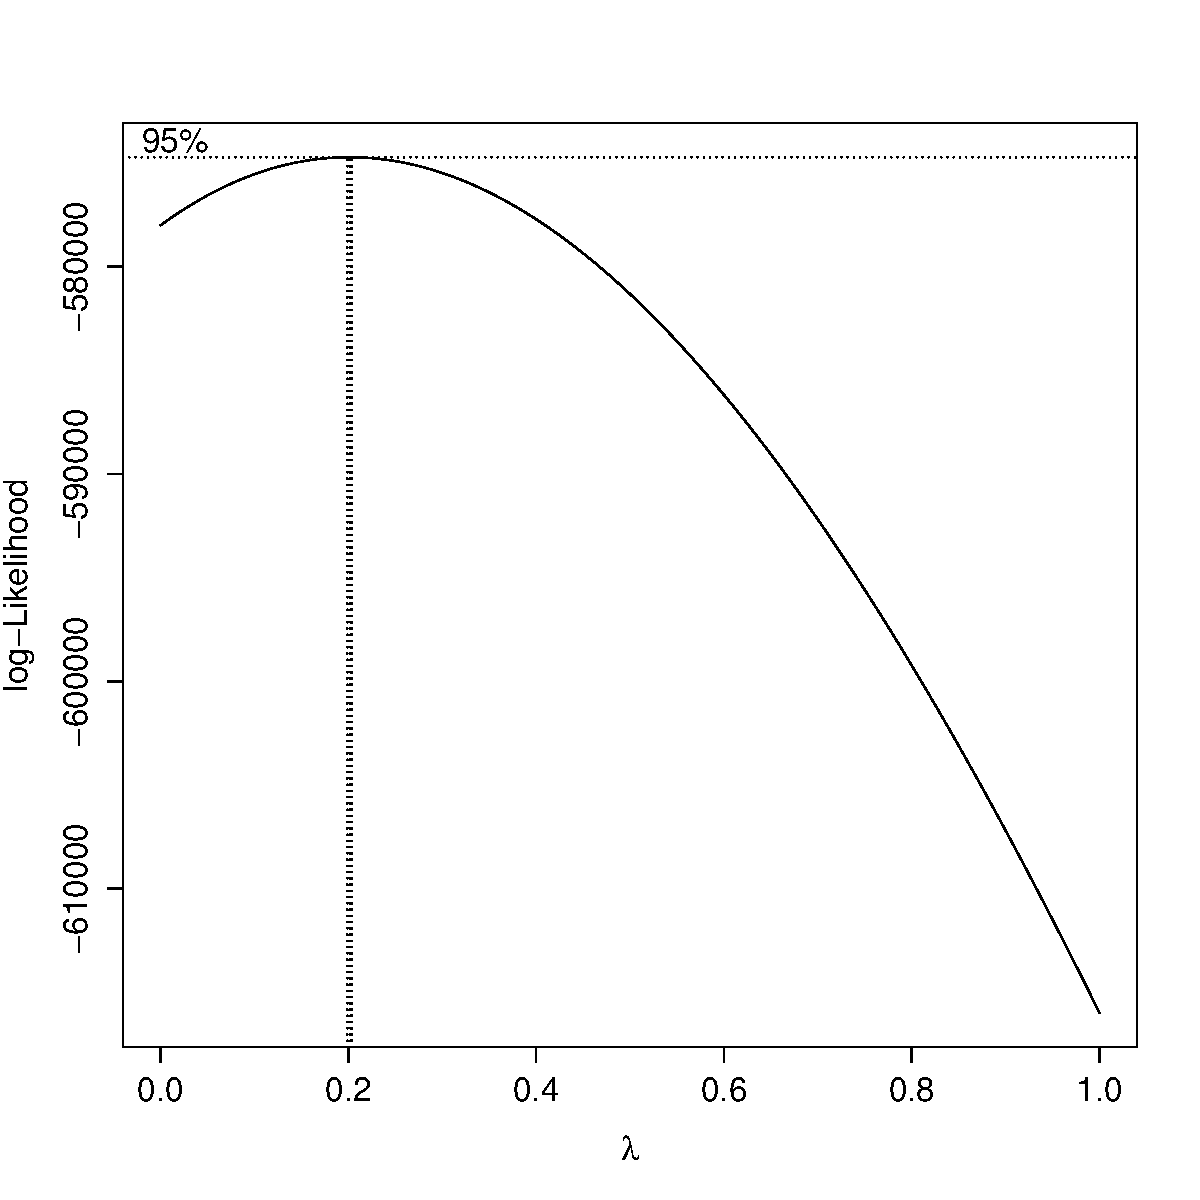
\includegraphics[width=0.4\linewidth]{figs/LogLikelihood-Backers.pdf}
	}
	\hspace{1cm}
	\subfigure[Value of $\lambda$ in regression model for predicting amount of funding] % caption for subfigure b
	{
		\label{fig:lambdaFunding}
		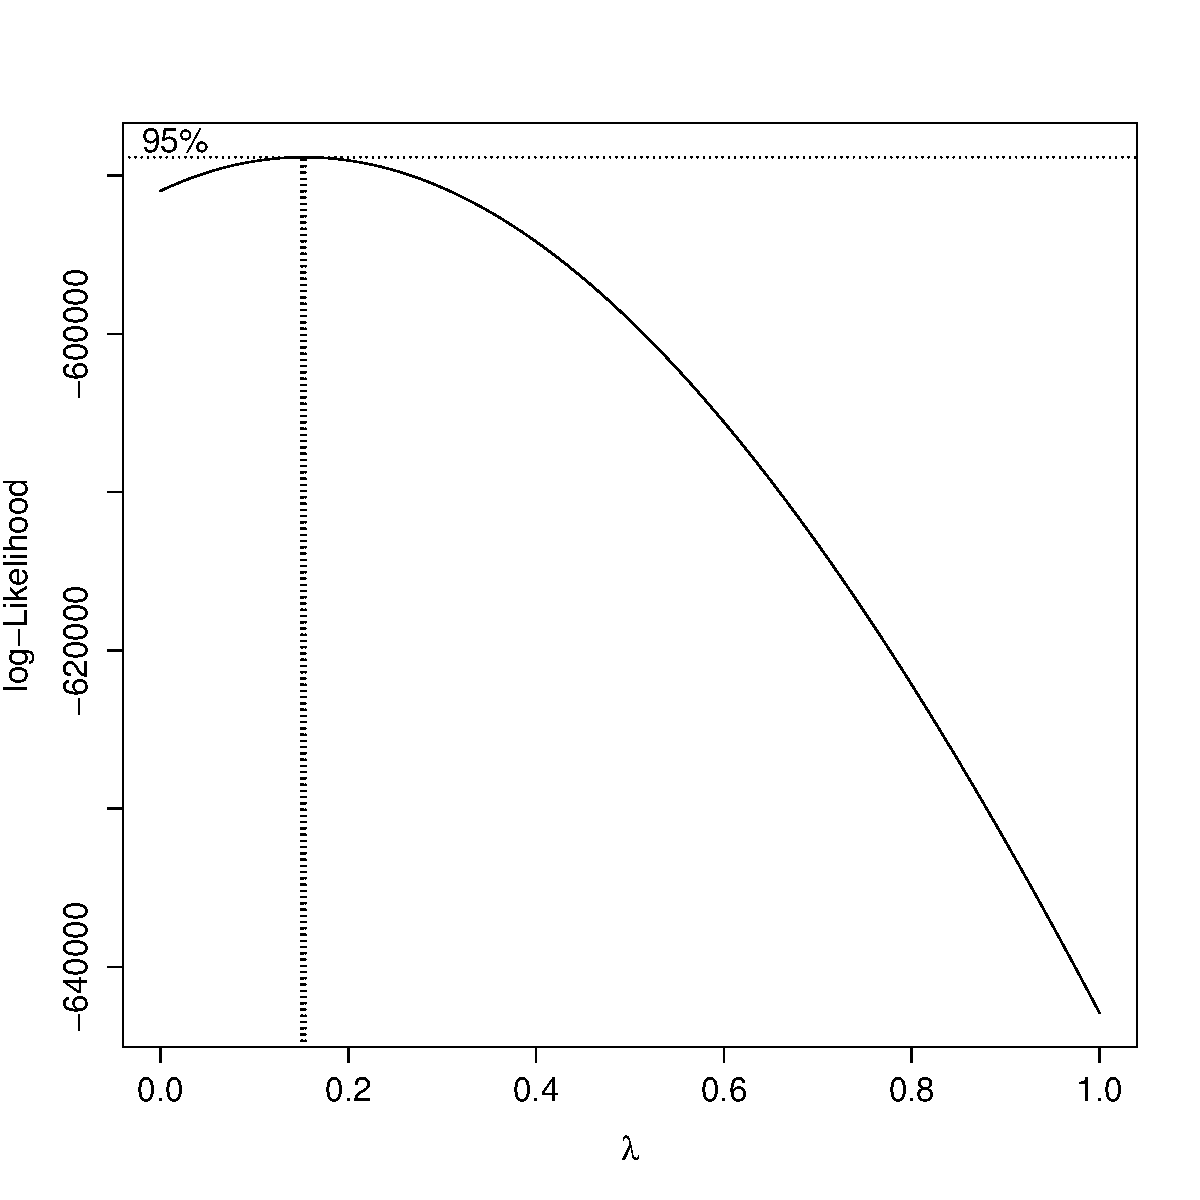
\includegraphics[width=0.4\linewidth]{figs/LogLikelihood-Funding.pdf}
	}
	\caption{Value of $\lambda$ in 2 models: predicting number of backers and the amount of funding}
	\label{fig:LambdaFig}
	\vspace{-10pt}
\end{figure*}
\begin{figure*}[!ht]
	\centering
	\subfigure[Predicting how many backers will back for a Kickstarter project] % caption for subfigure a
	{
		\label{fig:BackerRegressionResult}
		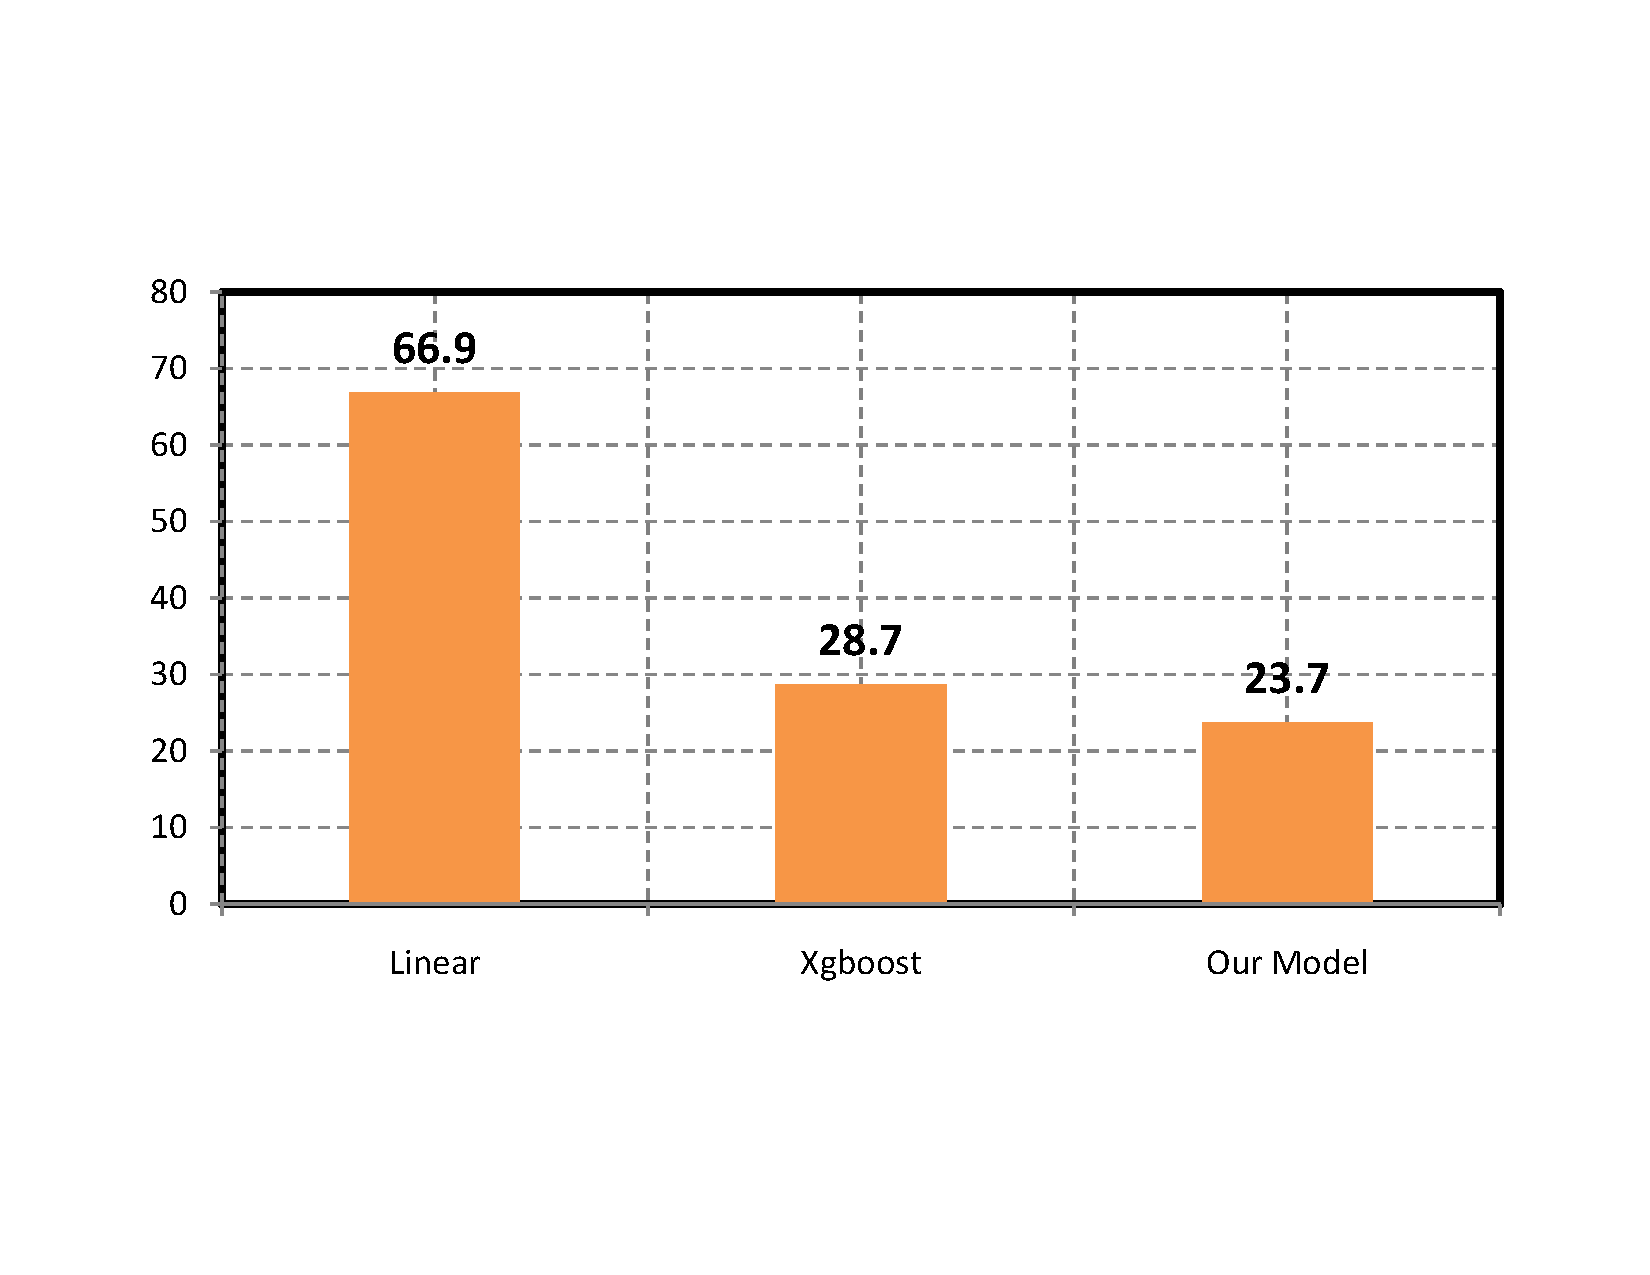
\includegraphics[width=0.4\linewidth]{figs/BackerRegressionResult.pdf}
	}
	\hspace{1cm}
	\subfigure[predicting how much funding a Kickstarter project can receive] % caption for subfigure b
	{
		\label{fig:FundingRegressionResult}
		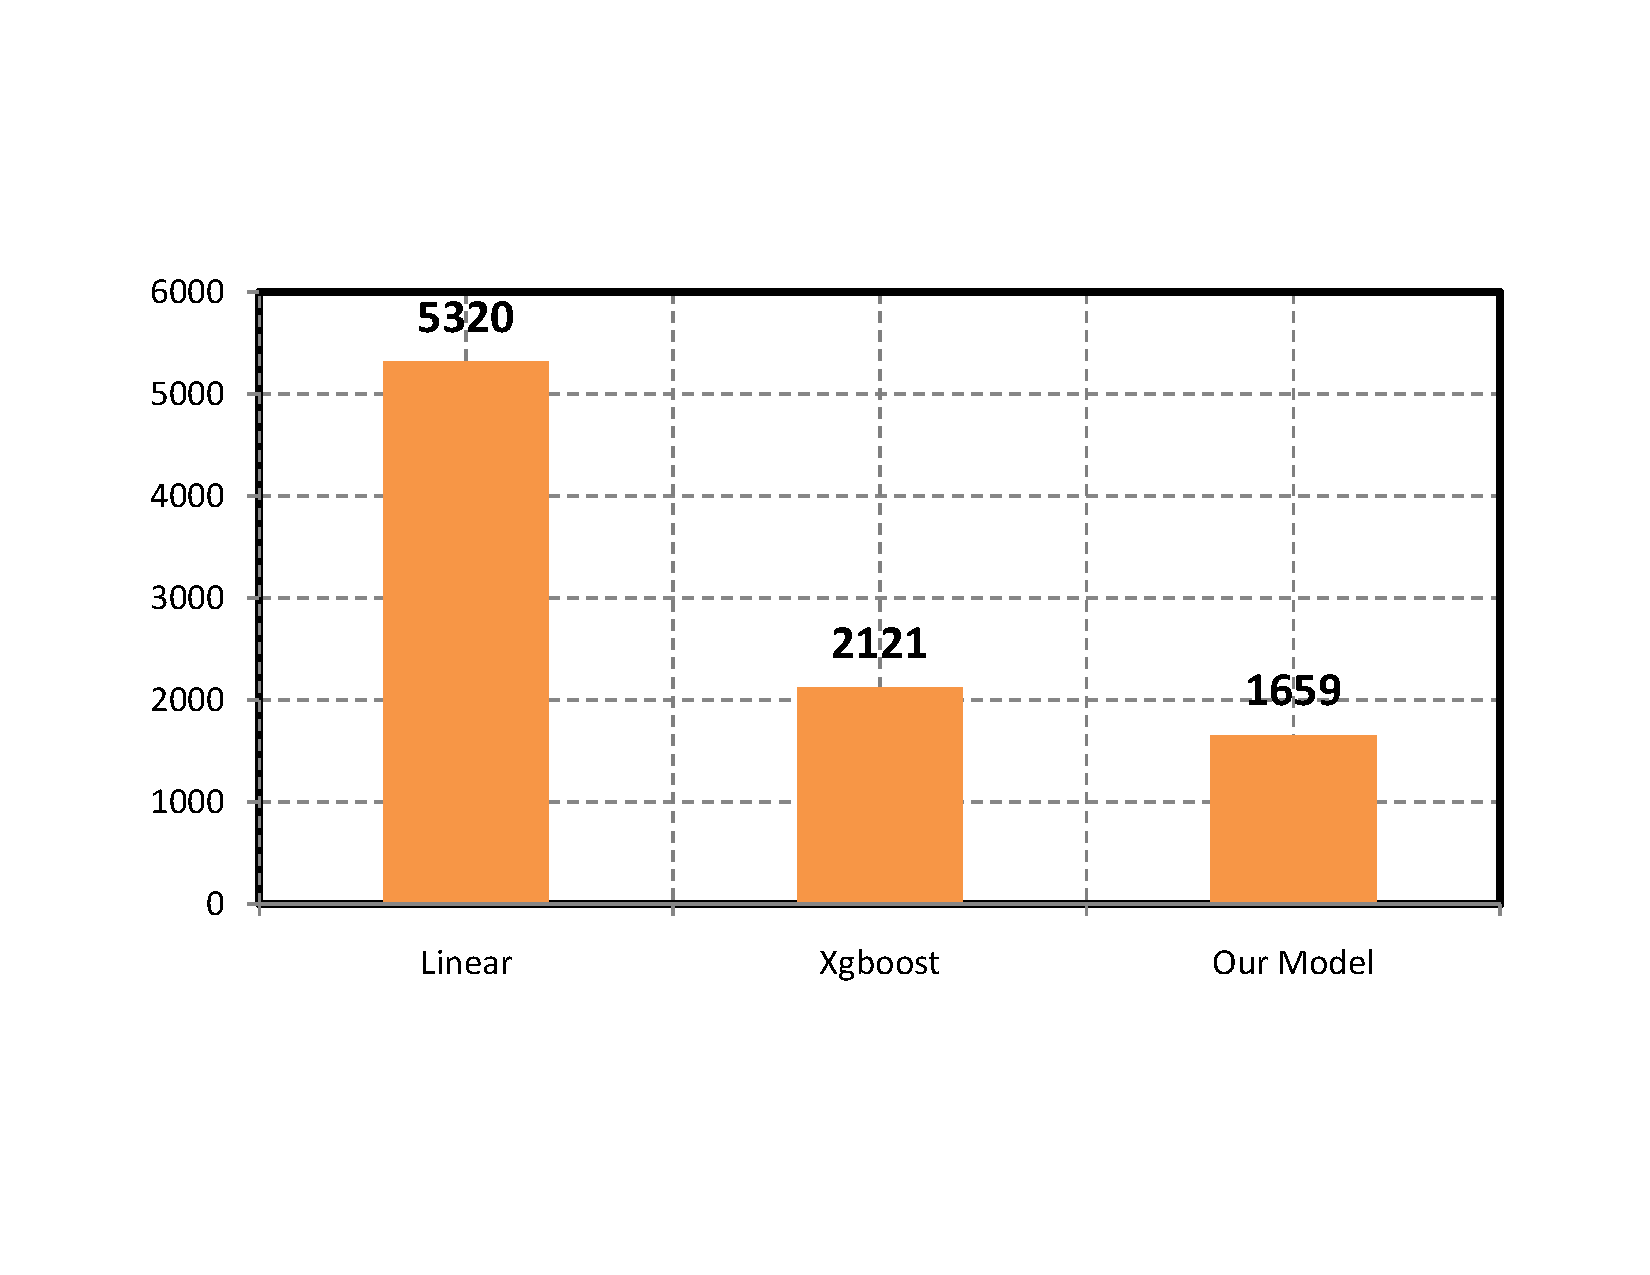
\includegraphics[width=0.4\linewidth]{figs/FundingRegressionResult.pdf}
	}
	\caption{RMSE of different models for (a) predicting how many backers will back for a Kickstarter project, and (b) predicting how much funding will a Kickstarter project receive}
	\label{fig:RegressionResult}
	\vspace{-10pt}
\end{figure*}
Figure \ref{fig:LambdaFig} shows the change of loglikelihood when varying the $\lambda$ value. For building the model to predict number of backers, we observed in Figure \ref{fig:lambdaBackers} that at $\lambda-0.2$, the loglikelihood function achieve the highest value. With regard to the model of predicting the amount of funding, it is shown in Figure \ref{fig:lambdaFunding} that we obtained the maximum value of loglikelihood when $\lambda = 0.18$. Hence, we set $\lambda = 0.2$ and 0.18 in the models of predicting number of backers and the amount of funding, respectively.

As a result, we fit the following model for predicting number of backers:
\begin{equation}
\label{equa:model1 }
\begin{aligned}
	Y_{backers}^{0.2} = \beta_0 + \beta^TX + \epsilon 
\end{aligned}
\end{equation}

And the model for predicting the amount of funding need to be fitted is as following:
\begin{equation}
\label{equa:model2}
\begin{aligned}
	Y_{funding}^{0.18} = \beta_0 + \beta^TX + \epsilon
\end{aligned}
\end{equation}
where $\epsilon$ is the random error and $\epsilon\sim N(0, \sigma^2)$ 

\textbf{Predicting how many backers will back for a Kickstarter project:} we fit our proposed model given in Equation (\ref{equa:model1 }). Then we compare the result with linear regression model and extreme gradient boosting for linear model. Figure \ref{fig:BackerRegressionResult} shows RMSE of 3 models for predicting how many backers will back for a Kickstarter project. We note that linear regression model obtained lowest result with RSME of 66.9. Boosting linear regression with Xgboost gained higher result with RSME of 28.7. However, comparing to these two models, our approach obtained the best result with lowest RSMSE of 23.7.

%\begin{figure}%[!ht]	
%	\centering
%	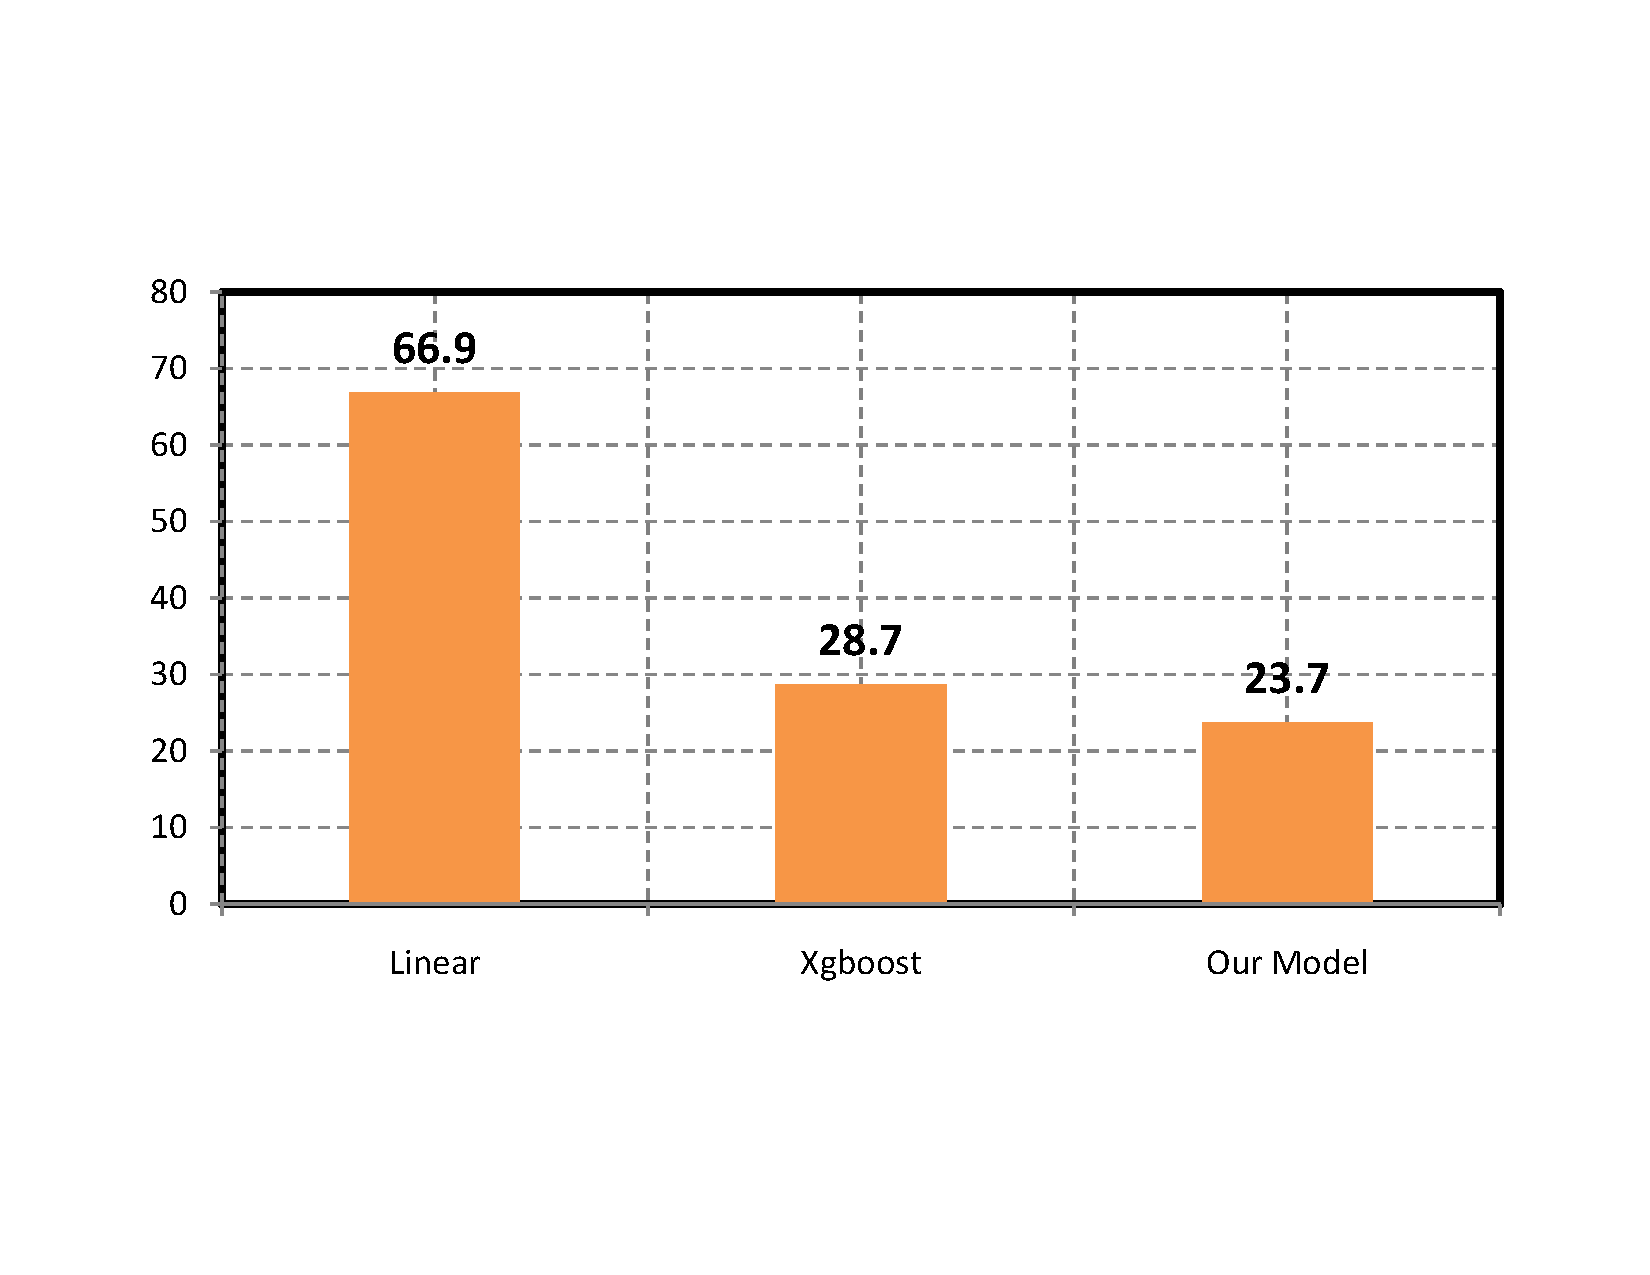
\includegraphics[width=\linewidth]{figs/BackerRegressionResult.pdf}
%	\caption{RMSE of different models for predicting how many backers will back for a Kickstarter project}
%	\label{fig:BackerRegressionResult}
%	\vspace{-10pt}
%\end{figure}

\textbf{Predicting the amount of funding a Kickstarter project can receive:} we fit our proposed model given in Equation (\ref{equa:model2}) to predict how much funding a Kickstarter project can be funded. We also compared our result with the results we got from linear boosting of Xgboost and linear regression. Figure \ref{fig:FundingRegressionResult} shows RMSE result of 3 models. We notice that our model outperformed linear regression and Xgboost for linear model with lowest RMSE of 1,659. This value is the average error of predicting the amount of funding for a Kickstarter project. 

%\begin{figure}%[!ht]
%	\centering
%	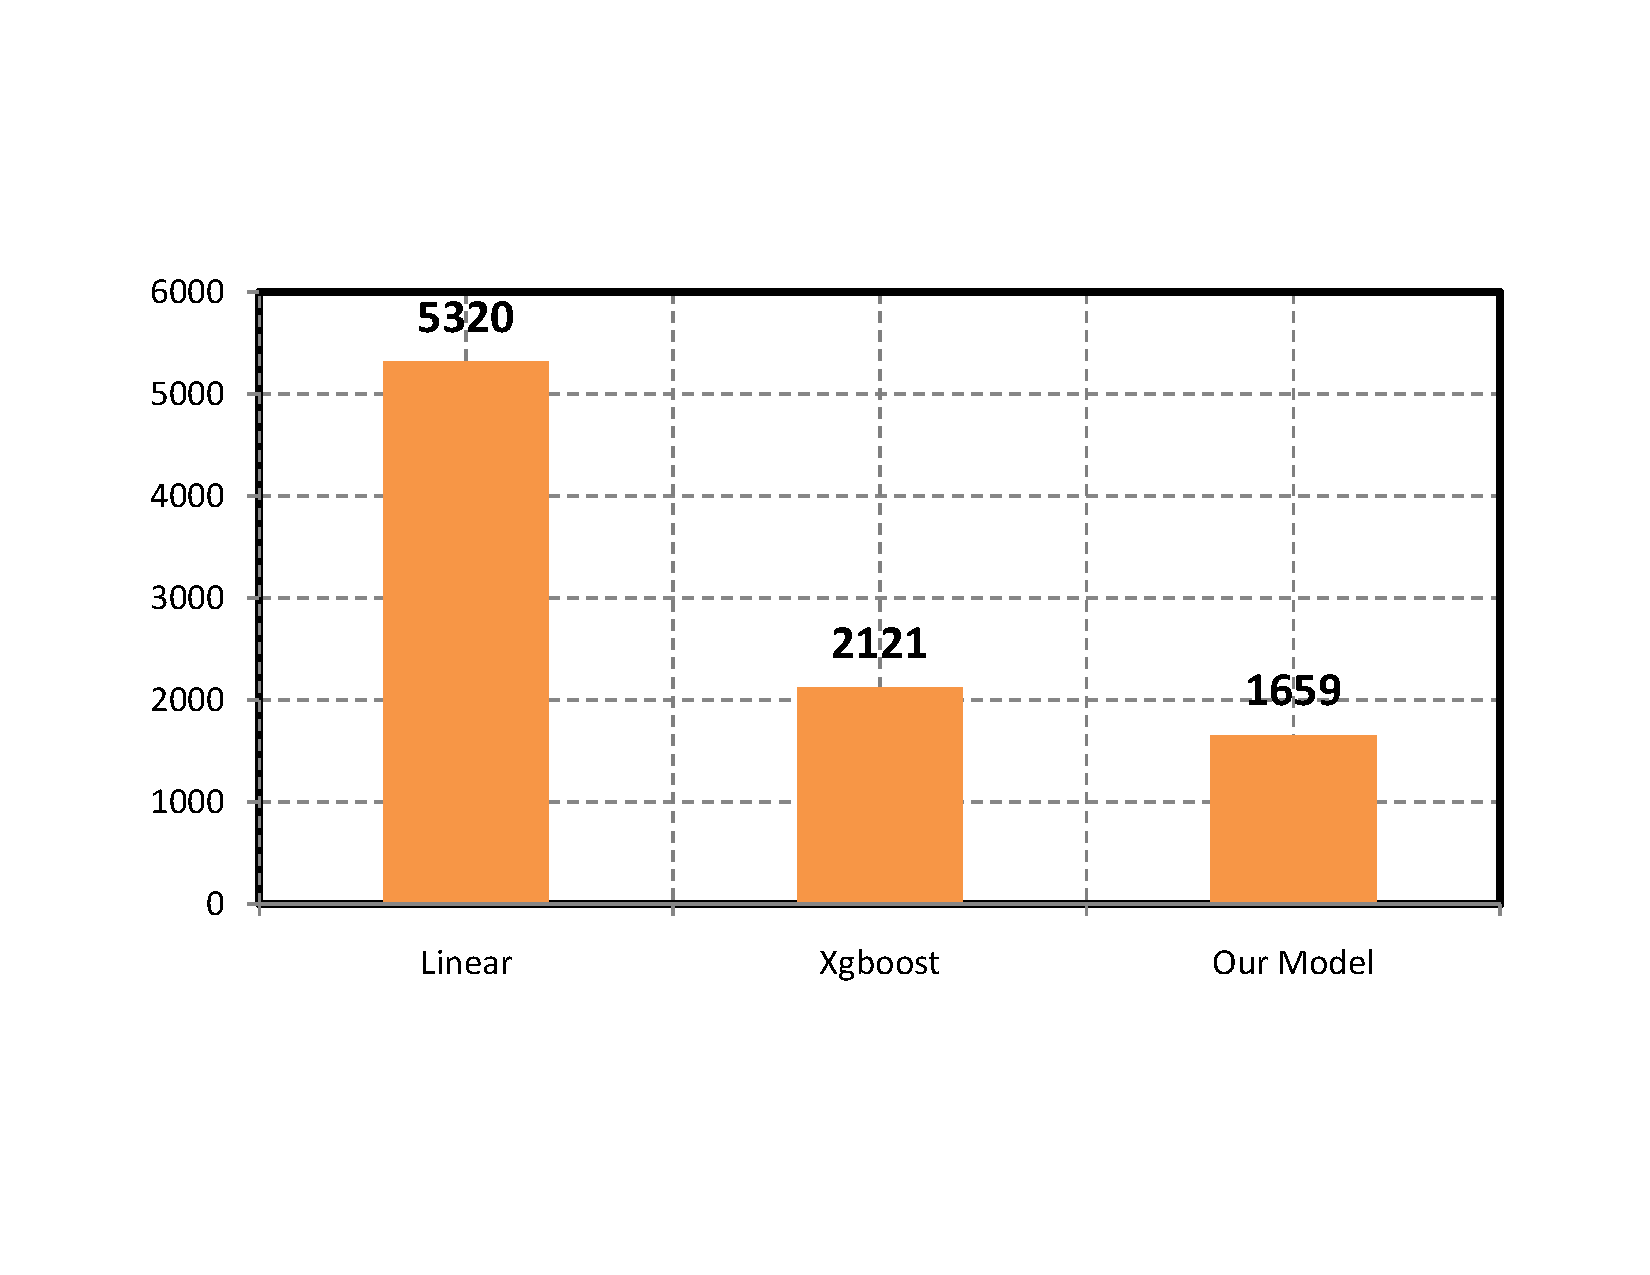
\includegraphics[width=\linewidth]{figs/FundingRegressionResult.pdf}
%	\caption{RMSE of different models for predicting how much funding will a Kickstarter project receive}
%	\label{fig:FundingRegressionResult}
%	\vspace{-10pt}
%\end{figure}

\section{Understanding the influence of factors toward the amount of funding}

\begin{table*}[!ht]
\centering
\caption{Coefficient of Features}
\label{coefficient-of-features}
\begin{tabular}{|l|r|l|r|}
\hline
Feature Name & Coefficient & Feature Name & Coefficient \\ \hline \hline
numProjectComments *** & 23539.09 & cbackedCategories  *** & 230.262 \\ \hline
numUpdates *** & 2816.502 & cbackedCategories  *** & 202.355 \\ \hline
cnumFbFriends *** & 1002.85 & cbackedCategories *** & 158.055 \\ \hline
numRewards *** & 951.701 & cnumBioSentence *** & 141.075 \\ \hline
Goal *** & 800.64 & numFaqs *** & 134.553 \\ \hline
previousProjectSuccessRate *** & 779.975 & cbackedCategories * & 89.731 \\ \hline
numVideos *** & 594.218 & numImages *** & 27.47 \\ \hline
smogBio *** & 444.779 & cbackedCategories *** & 13.272 \\ \hline
cbackedCategories *** & 429.861 & cwebsiteCount *** & 7.455 \\ \hline
backedProjectSuccessfulRate *** & 428.13 & ctwitterConnected *** & -0.5 \\ \hline
smogMain *** & 341.549 & cbackedCategories ** & -61.033 \\ \hline
numMainSentences  *** & 335.187 & cyoutubeConnected  *** & -183.622 \\ \hline
Category  *** & 293.621 & cbackedCategories ** & -249.037 \\ \hline
cbackedCategories  *** & 291.544 & cfacebookConnected *** & -643.742 \\ \hline
cbackedCategories  *** & 264.193 & cbackedCategories *** & -697.825 \\ \hline
cnumCreatorComment  * & 246.34 & cbackedCategories *** & -847.89 \\ \hline
cbackedCategories  *** & 240.012 & cnumCreated *** & -1915.6 \\ \hline
\end{tabular}
\end{table*}

Table \ref{coefficient-of-features} explains which features have more influence on determining the amount of funding. * represent the significance of $\alpha$(*: 0.05, **: 0.01, ***: 0.001). Larger value in coefficient is more impact on prediction of the amount of funding. As table shows, the number of project comments is out-numbering other features as value of 23,540 which is a lot greater than the second ranking attribute of the number updates having 2,817. It is important to response on backers by project owners explaining communication between them is essential element of success.

Besides, some of features have negative relation with the amount of funding. The attribute which has the worst relationship with response is how many times project the creator has published in the past. This explains that backers consider the creator who made a lot in the past tends not to be successful to be funded overtime. The next following features the number of categories the creator has been made in the past. The creator did not focus on one specific area but extend its territories to several realm. Backers might suspect that the creator does not possess specialty on specific object. Backers are likely to avoid the project which project owner has no specialty.

